\documentclass[12pt]{article}

% Packages
\usepackage{graphicx}
\usepackage{booktabs}
\usepackage{amsmath}
\usepackage{float}
\usepackage{subcaption}
\usepackage{geometry}
\usepackage{hyperref}
\usepackage{caption}

% Page setup
\geometry{a4paper, margin=1in}

% Document info
\title{Rainfall Forecasting in Selangor Using Machine Learning Techniques}
\author{Author Name}
\date{\today}

\begin{document}
% Chapter 3: Methodology
\chapter{Methodology}
\label{chap:methodology}

This chapter explain detailed methodology used for forecasting rainfall in Selangor using machine learning techniques. The process involve data acquisition, preprocessing, feature engineering, model implementation and evaluation framework.

\section{Data Acquisition and Integration}
\label{sec:data_acquisition}

The dataset for this study was obtained from official weather station records in Selangor, Malaysia. Two CSV files were used for this research:

\begin{itemize}
    \item \texttt{230731665812CCD\_weekly1.csv}: Contains 470 records of weekly weather data from 2012-2021
    \item \texttt{230731450378CCD\_weekly2.csv}: Validation duplicate used for data integrity checking
\end{itemize}

Data loading was implemented with robust error handling and validation checks to ensure data integrity. The dataset contains following features:

\begin{table}[h]
\centering
\caption{Dataset Features}
\label{tab:dataset_features}
\begin{tabular}{|l|l|p{8cm}|}
\hline
\textbf{Feature} & \textbf{Unit} & \textbf{Description} \\
\hline
Date & YYYY-MM-DD & Date of record \\
\hline
Precipitation\_mm & mm & Weekly precipitation amount (target variable) \\
\hline
Temp\_avg & °C & Average weekly temperature \\
\hline
Relative\_Humidity & \% & Average weekly relative humidity \\
\hline
Wind\_kmh & km/h & Average weekly wind speed \\
\hline
Week\_Number & 1-52 & Week number in year \\
\hline
Year & YYYY & Year of record \\
\hline
\end{tabular}
\end{table}

To ensure data reliability, duplicate detection was performed when merging the two CSV files. This approach is cost-efficient as it use existing datasets without need for external API calls.

\section{Data Preprocessing Pipeline}
\label{sec:data_preprocessing}

A comprehensive preprocessing pipeline was implemented to prepare the data for model training. This pipeline include data cleaning, feature engineering, normalization, and data splitting.

\subsection{Data Cleaning}
\label{subsec:data_cleaning}

\subsubsection{Missing Value Handling}
\label{subsubsec:missing_values}

Missing values were handled using mean imputation with \texttt{pandas.fillna()} method. Validation checks were performed before and after imputation to ensure data integrity. All operations were logged for traceability. The proportion of missing values was low ($<2\%$), making mean imputation a suitable approach.

\subsubsection{Outlier Detection and Removal}
\label{subsubsec:outlier_detection}

An Interquartile Range (IQR) based method was employed to detect and remove outliers. This non-parametric approach is robust to non-normal distributions and less sensitive to extreme values than standard deviation-based methods. The following acceptable ranges were established based on domain knowledge:

\begin{itemize}
    \item Temperature: 20-35°C
    \item Humidity: 0-100\%
    \item Wind speed: 0-15 km/h
    \item Precipitation: 0-400mm
\end{itemize}

The IQR method was implemented as follows:

\begin{equation}
Q_1 = \text{25th percentile}, \quad Q_3 = \text{75th percentile}
\end{equation}

\begin{equation}
IQR = Q_3 - Q_1
\end{equation}

\begin{equation}
\text{Lower bound} = Q_1 - 1.5 \times IQR, \quad \text{Upper bound} = Q_3 + 1.5 \times IQR
\end{equation}

Values outside these bounds were flagged as outliers and treated according to the following rules:
\begin{itemize}
    \item Values slightly outside bounds ($< 3 \times IQR$) were capped at the boundary values
    \item Extreme outliers ($> 3 \times IQR$) were removed to prevent model bias
\end{itemize}

\subsection{Feature Engineering}
\label{subsec:feature_engineering}

To enhance model performance, several new features were created:

\subsubsection{Lag Variables}
\label{subsubsec:lag_variables}

Lag variables capture the influence of previous time periods on the current prediction:
\begin{itemize}
    \item \texttt{precipitation\_lag\_1}: Previous week's precipitation
    \item \texttt{temp\_lag\_1}: Previous week's temperature
    \item \texttt{humidity\_lag\_1}: Previous week's humidity
\end{itemize}

These variables were created using pandas shift() operation:
\begin{verbatim}
df['precipitation_lag_1'] = df['Precipitation_mm'].shift(1)
\end{verbatim}

\subsubsection{Moving Averages}
\label{subsubsec:moving_averages}

Moving averages smooth out short-term fluctuations and highlight longer-term trends:
\begin{itemize}
    \item \texttt{precipitation\_ma\_3}: 3-week moving average of precipitation
    \item \texttt{temp\_ma\_4}: 4-week moving average of temperature
    \item \texttt{humidity\_ma\_3}: 3-week moving average of humidity
\end{itemize}

Implementation:
\begin{verbatim}
df['precipitation_ma_3'] = df['Precipitation_mm'].rolling(window=3).mean()
\end{verbatim}

\subsubsection{Seasonal Features}
\label{subsubsec:seasonal_features}

To capture the seasonal patterns of rainfall in Selangor, the following binary indicators were created:
\begin{itemize}
    \item \texttt{monsoon\_season}: Boolean flag for Northeast Monsoon (Oct-Dec) and Southwest Monsoon (Apr)
    \item \texttt{dry\_season}: Boolean flag for drier months (Jun-Aug)
\end{itemize}

Additionally, cyclical encoding was applied to the \texttt{week\_of\_year} feature using sine and cosine transformations to preserve the cyclical nature of weeks:

\begin{equation}
\text{week\_sin} = \sin\left(\frac{2\pi \times \text{week}}{52}\right)
\end{equation}

\begin{equation}
\text{week\_cos} = \cos\left(\frac{2\pi \times \text{week}}{52}\right)
\end{equation}

\subsubsection{Interaction Features}
\label{subsubsec:interaction_features}

Interaction features capture the combined effect of multiple variables:
\begin{itemize}
    \item \texttt{temp\_humidity\_interaction}: Temp\_avg $\times$ Relative\_Humidity
    \item \texttt{wind\_precipitation\_ratio}: Wind\_kmh / (Precipitation\_mm + 1)
\end{itemize}

The addition of 1 to precipitation prevents division by zero.

\subsection{Normalization}
\label{subsec:normalization}

All features were scaled to the [0,1] range using MinMaxScaler from scikit-learn:

\begin{equation}
X_{scaled} = \frac{X - X_{min}}{X_{max} - X_{min}}
\end{equation}

Separate scalers were used for features and the target variable to facilitate inverse transformation during prediction. Both scalers were saved for future use:

\begin{verbatim}
from sklearn.preprocessing import MinMaxScaler
feature_scaler = MinMaxScaler()
X_train_scaled = feature_scaler.fit_transform(X_train)
X_test_scaled = feature_scaler.transform(X_test)

target_scaler = MinMaxScaler()
y_train_scaled = target_scaler.fit_transform(y_train.reshape(-1, 1))
y_test_scaled = target_scaler.transform(y_test.reshape(-1, 1))

# Save scalers
joblib.dump(feature_scaler, 'models/scalers/feature_scaler.pkl')
joblib.dump(target_scaler, 'models/scalers/target_scaler.pkl')
\end{verbatim}

\subsection{Data Splitting}
\label{subsec:data_splitting}

The dataset was split into training (80\%, 376 records) and testing (20\%, 94 records) sets using scikit-learn's \texttt{train\_test\_split} function. The splitting process maintained chronological order due to the time-series nature of the data, ensuring that all test data points come after training data points. Additionally, stratification by year was implemented to ensure representative data across all years:

\begin{verbatim}
from sklearn.model_selection import train_test_split
# Sort data chronologically first
df = df.sort_values('Date')
# Extract year for stratification
year_strata = df['Year']
# Perform split
X_train, X_test, y_train, y_test = train_test_split(
    X, y, test_size=0.2, random_state=42, 
    shuffle=False, stratify=year_strata
)
\end{verbatim}

\section{Model Implementation}
\label{sec:model_implementation}

Six different models were implemented to forecast rainfall in Selangor. Each model was chosen to capture different aspects of the rainfall patterns.

\subsection{Artificial Neural Network (ANN)}
\label{subsec:ann}

A sequential neural network was implemented using Keras with TensorFlow backend:

\begin{verbatim}
from tensorflow import keras
from tensorflow.keras.layers import Dense, Dropout
from tensorflow.keras.models import Sequential

def create_ann_model(input_dim):
    model = Sequential()
    model.add(Dense(64, activation='relu', input_dim=input_dim))
    model.add(Dropout(0.2))
    model.add(Dense(32, activation='relu'))
    model.add(Dropout(0.2))
    model.add(Dense(1, activation='linear'))
    
    model.compile(
        optimizer=keras.optimizers.Adam(learning_rate=0.001),
        loss='mean_squared_error'
    )
    return model
\end{verbatim}

The model architecture consists of:
\begin{itemize}
    \item Input layer with dimensionality matching the number of features
    \item First hidden layer with 64 neurons and ReLU activation
    \item Dropout layer (rate=0.2) for regularization
    \item Second hidden layer with 32 neurons and ReLU activation
    \item Another dropout layer (rate=0.2)
    \item Output layer with a single neuron and linear activation (for regression)
\end{itemize}

The model was compiled with Adam optimizer and mean squared error loss function.

\subsection{Multiple Linear Regression (MLR)}
\label{subsec:mlr}

Multiple Linear Regression served as a baseline model:

\begin{verbatim}
from sklearn.linear_model import LinearRegression
from sklearn.feature_selection import RFE

def create_mlr_model(n_features_to_select=10):
    base_model = LinearRegression()
    selector = RFE(estimator=base_model, n_features_to_select=n_features_to_select)
    return selector
\end{verbatim}

Recursive Feature Elimination (RFE) was employed to select the most important features, reducing model complexity and mitigating multicollinearity. Assumptions of linearity, homoscedasticity, and normality were tested:

\begin{itemize}
    \item Linearity: Scatter plots of each feature vs. target
    \item Homoscedasticity: Residuals vs. predicted values plot
    \item Normality: Q-Q plot of residuals
\end{itemize}

\subsection{K-Nearest Neighbors (KNN)}
\label{subsec:knn}

The KNN regressor was implemented as follows:

\begin{verbatim}
from sklearn.neighbors import KNeighborsRegressor

def create_knn_model(n_neighbors=5, weights='uniform', 
                    metric='euclidean'):
    model = KNeighborsRegressor(
        n_neighbors=n_neighbors,
        weights=weights,
        metric=metric
    )
    return model
\end{verbatim}

KNN makes predictions based on the average of the k nearest training samples, making it effective for capturing local patterns in the data.

\subsection{Random Forest (RF)}
\label{subsec:rf}

Random Forest, an ensemble of decision trees, was implemented:

\begin{verbatim}
from sklearn.ensemble import RandomForestRegressor

def create_rf_model(n_estimators=100, max_depth=None, 
                   min_samples_split=2, min_samples_leaf=1,
                   max_features='auto', random_state=42):
    model = RandomForestRegressor(
        n_estimators=n_estimators,
        max_depth=max_depth,
        min_samples_split=min_samples_split,
        min_samples_leaf=min_samples_leaf,
        max_features=max_features,
        random_state=random_state,
        n_jobs=-1  # Parallel processing
    )
    return model
\end{verbatim}

Random Forest is well-suited for capturing non-linear relationships and providing feature importance metrics.

\subsection{Gradient Boosting (XGBoost)}
\label{subsec:xgboost}

XGBoost, an optimized gradient boosting implementation, was used:

\begin{verbatim}
import xgboost as xgb

def create_xgb_model(n_estimators=100, learning_rate=0.1, 
                    max_depth=3, subsample=1.0, 
                    colsample_bytree=1.0, reg_alpha=0,
                    reg_lambda=1, random_state=42):
    model = xgb.XGBRegressor(
        n_estimators=n_estimators,
        learning_rate=learning_rate,
        max_depth=max_depth,
        subsample=subsample,
        colsample_bytree=colsample_bytree,
        reg_alpha=reg_alpha,
        reg_lambda=reg_lambda,
        random_state=random_state,
        n_jobs=-1
    )
    return model
\end{verbatim}

XGBoost builds trees sequentially, with each tree correcting the errors of the previous ones, making it effective for capturing complex patterns.

\subsection{ARIMA}
\label{subsec:arima}

Autoregressive Integrated Moving Average (ARIMA) model was implemented for time series forecasting:

\begin{verbatim}
from statsmodels.tsa.arima.model import ARIMA

def create_arima_model(p=1, d=1, q=1):
    model = ARIMA(order=(p, d, q))
    return model
\end{verbatim}

Before implementing ARIMA, stationarity was tested using the Augmented Dickey-Fuller test. Autocorrelation Function (ACF) and Partial Autocorrelation Function (PACF) plots were analyzed to identify appropriate p and q parameters.

\section{Hyperparameter Tuning}
\label{sec:hyperparameter_tuning}

Hyperparameter optimization was performed to maximize model performance.

\subsection{GridSearchCV for Traditional Models}
\label{subsec:gridsearchcv}

For KNN, Random Forest, and XGBoost models, GridSearchCV was used to systematically explore the hyperparameter space:

\begin{verbatim}
from sklearn.model_selection import GridSearchCV

# Example for Random Forest
param_grid = {
    'n_estimators': [100, 200, 300, 500],
    'max_depth': [10, 20, 30, 50, None],
    'min_samples_split': [2, 5, 10],
    'min_samples_leaf': [1, 2, 4],
    'max_features': ['auto', 'sqrt', 'log2']
}

rf = RandomForestRegressor(random_state=42)
grid_search = GridSearchCV(
    estimator=rf,
    param_grid=param_grid,
    cv=5,  # 5-fold cross-validation
    scoring='neg_mean_squared_error',
    n_jobs=-1,  # Parallel processing
    verbose=2
)

grid_search.fit(X_train_scaled, y_train_scaled)
best_rf = grid_search.best_estimator_
\end{verbatim}

The hyperparameter search spaces for each model were as follows:

\subsubsection{KNN Hyperparameters}
\begin{itemize}
    \item \texttt{n\_neighbors}: [3, 5, 7, 9, 11, 15]
    \item \texttt{weights}: ['uniform', 'distance']
    \item \texttt{metric}: ['euclidean', 'manhattan', 'minkowski']
    \item \texttt{p}: [1, 2] (for minkowski metric)
\end{itemize}

\subsubsection{Random Forest Hyperparameters}
\begin{itemize}
    \item \texttt{n\_estimators}: [100, 200, 300, 500]
    \item \texttt{max\_depth}: [10, 20, 30, 50, None]
    \item \texttt{min\_samples\_split}: [2, 5, 10]
    \item \texttt{min\_samples\_leaf}: [1, 2, 4]
    \item \texttt{max\_features}: ['auto', 'sqrt', 'log2']
\end{itemize}

\subsubsection{XGBoost Hyperparameters}
\begin{itemize}
    \item \texttt{n\_estimators}: [100, 200, 300]
    \item \texttt{learning\_rate}: [0.01, 0.1, 0.2]
    \item \texttt{max\_depth}: [3, 6, 9]
    \item \texttt{subsample}: [0.8, 0.9, 1.0]
    \item \texttt{colsample\_bytree}: [0.8, 0.9, 1.0]
    \item \texttt{reg\_alpha}: [0, 0.1, 1]
    \item \texttt{reg\_lambda}: [1, 1.5, 2]
\end{itemize}

\subsection{Optuna for Neural Networks}
\label{subsec:optuna}

For the ANN model, Optuna was employed for more efficient hyperparameter optimization:

\begin{verbatim}
import optuna
from tensorflow import keras

def create_model(trial):
    n_layers = trial.suggest_int('n_layers', 2, 4)
    n_units = [trial.suggest_categorical(f'n_units_l{i}', 
                                        [32, 64, 128]) 
              for i in range(n_layers)]
    activation = trial.suggest_categorical('activation', 
                                        ['relu', 'tanh', 'sigmoid'])
    learning_rate = trial.suggest_loguniform('learning_rate', 
                                           1e-3, 1e-1)
    dropout_rate = trial.suggest_uniform('dropout_rate', 0.1, 0.3)
    
    model = keras.Sequential()
    model.add(keras.layers.Dense(n_units[0], activation=activation, 
                               input_dim=X_train_scaled.shape[1]))
    model.add(keras.layers.Dropout(dropout_rate))
    
    for i in range(1, n_layers):
        model.add(keras.layers.Dense(n_units[i], activation=activation))
        model.add(keras.layers.Dropout(dropout_rate))
    
    model.add(keras.layers.Dense(1, activation='linear'))
    
    model.compile(
        optimizer=keras.optimizers.Adam(learning_rate=learning_rate),
        loss='mean_squared_error'
    )
    
    return model

def objective(trial):
    model = create_model(trial)
    batch_size = trial.suggest_categorical('batch_size', [16, 32, 64])
    epochs = trial.suggest_categorical('epochs', [50, 100, 200])
    
    # Early stopping to prevent overfitting
    early_stopping = keras.callbacks.EarlyStopping(
        monitor='val_loss',
        patience=20,
        restore_best_weights=True
    )
    
    history = model.fit(
        X_train_scaled, y_train_scaled,
        epochs=epochs,
        batch_size=batch_size,
        validation_split=0.2,
        callbacks=[early_stopping],
        verbose=0
    )
    
    val_loss = min(history.history['val_loss'])
    return val_loss

study = optuna.create_study(direction='minimize')
study.optimize(objective, n_trials=30)

best_params = study.best_params
best_ann = create_model(optuna.trial.FixedTrial(best_params))
\end{verbatim}

The Optuna search space included:
\begin{itemize}
    \item Number of layers: 2-4
    \item Neurons per layer: [32, 64, 128]
    \item Activation functions: ['relu', 'tanh', 'sigmoid']
    \item Learning rate: 0.001-0.1 (log-uniform)
    \item Batch size: [16, 32, 64]
    \item Epochs: [50, 100, 200]
    \item Dropout rate: 0.1-0.3 (uniform)
\end{itemize}

\subsection{ARIMA Parameter Selection}
\label{subsec:arima_parameter}

For the ARIMA model, parameters were selected based on statistical tests and information criteria:

\begin{verbatim}
from statsmodels.tsa.stattools import adfuller
from statsmodels.graphics.tsaplots import plot_acf, plot_pacf
import itertools
import warnings
warnings.filterwarnings('ignore')

# Test for stationarity
def adf_test(timeseries):
    result = adfuller(timeseries)
    print(f'ADF Statistic: {result[0]}')
    print(f'p-value: {result[1]}')
    for key, value in result[4].items():
        print(f'Critical Value ({key}): {value}')
    if result[1] <= 0.05:
        print("Stationary")
    else:
        print("Non-Stationary")

# Find optimal ARIMA parameters
def find_best_arima_params(data, p_range, d_range, q_range):
    best_aic = float('inf')
    best_params = None
    
    for p, d, q in itertools.product(p_range, d_range, q_range):
        try:
            model = ARIMA(data, order=(p, d, q))
            results = model.fit()
            aic = results.aic
            
            if aic < best_aic:
                best_aic = aic
                best_params = (p, d, q)
                
        except Exception as e:
            continue
    
    return best_params, best_aic

# Grid search for ARIMA parameters
p_range = range(0, 4)
d_range = range(0, 2)
q_range = range(0, 4)
best_params, best_aic = find_best_arima_params(
    y_train, p_range, d_range, q_range
)
print(f"Best ARIMA parameters: {best_params} with AIC: {best_aic}")
\end{verbatim}

\section{Model Evaluation Framework}
\label{sec:evaluation_framework}

A standardized evaluation framework was implemented to assess and compare model performance.

\subsection{Performance Metrics}
\label{subsec:performance_metrics}

The following metrics were used for model evaluation:

\begin{itemize}
    \item Mean Absolute Error (MAE):
    \begin{equation}
    \text{MAE} = \frac{1}{n}\sum_{i=1}^{n}|y_i - \hat{y}_i|
    \end{equation}
    
    \item Mean Squared Error (MSE):
    \begin{equation}
    \text{MSE} = \frac{1}{n}\sum_{i=1}^{n}(y_i - \hat{y}_i)^2
    \end{equation}
    
    \item Root Mean Squared Error (RMSE):
    \begin{equation}
    \text{RMSE} = \sqrt{\frac{1}{n}\sum_{i=1}^{n}(y_i - \hat{y}_i)^2}
    \end{equation}
    
    \item Coefficient of Determination (R²):
    \begin{equation}
    R^2 = 1 - \frac{\sum_{i=1}^{n}(y_i - \hat{y}_i)^2}{\sum_{i=1}^{n}(y_i - \bar{y})^2}
    \end{equation}
\end{itemize}

where $y_i$ are the actual values, $\hat{y}_i$ are the predicted values, and $\bar{y}$ is the mean of the actual values.

\subsection{Evaluation Function}
\label{subsec:evaluation_function}

A standardized evaluation function was implemented to calculate all metrics:

\begin{verbatim}
from sklearn.metrics import mean_absolute_error, mean_squared_error, r2_score
import numpy as np

def evaluate_model(y_true, y_pred, model_name):
    mae = mean_absolute_error(y_true, y_pred)
    mse = mean_squared_error(y_true, y_pred)
    rmse = np.sqrt(mse)
    r2 = r2_score(y_true, y_pred)
    
    results = {
        'Model': model_name,
        'MAE': mae,
        'MSE': mse,
        'RMSE': rmse,
        'R²': r2
    }
    
    return results
\end{verbatim}

\subsection{Automated Evaluation Pipeline}
\label{subsec:evaluation_pipeline}

An automated pipeline was created to evaluate all models and store results in a pandas DataFrame:

\begin{verbatim}
import pandas as pd

def evaluate_all_models(models, X_test_scaled, y_test_scaled, target_scaler):
    results_list = []
    predictions = {}
    
    for name, model in models.items():
        if name == 'ARIMA':
            # Special handling for ARIMA
            pred = model.forecast(len(y_test_scaled))
            y_pred_scaled = pred.reshape(-1, 1)
        else:
            y_pred_scaled = model.predict(X_test_scaled)
            if isinstance(y_pred_scaled, np.ndarray) and y_pred_scaled.ndim == 1:
                y_pred_scaled = y_pred_scaled.reshape(-1, 1)
        
        # Inverse transform to original scale
        y_test = target_scaler.inverse_transform(y_test_scaled)
        y_pred = target_scaler.inverse_transform(y_pred_scaled)
        
        # Store predictions for later visualization
        predictions[name] = y_pred.ravel()
        
        # Evaluate model
        result = evaluate_model(y_test, y_pred, name)
        results_list.append(result)
    
    # Create DataFrame from results
    results_df = pd.DataFrame(results_list)
    
    return results_df, predictions
\end{verbatim}

\subsection{Statistical Significance Testing}
\label{subsec:significance_testing}

Paired t-tests were performed to determine if the differences in model performance were statistically significant:

\begin{verbatim}
from scipy.stats import ttest_rel

def compare_models_statistically(models, X_test_scaled, y_test_scaled, 
                               target_scaler, alpha=0.05):
    model_names = list(models.keys())
    n_models = len(model_names)
    p_values = np.zeros((n_models, n_models))
    
    # Get predictions from each model
    predictions = {}
    for name, model in models.items():
        if name == 'ARIMA':
            pred = model.forecast(len(y_test_scaled))
            y_pred_scaled = pred.reshape(-1, 1)
        else:
            y_pred_scaled = model.predict(X_test_scaled)
            if isinstance(y_pred_scaled, np.ndarray) and y_pred_scaled.ndim == 1:
                y_pred_scaled = y_pred_scaled.reshape(-1, 1)
        
        # Inverse transform
        y_pred = target_scaler.inverse_transform(y_pred_scaled)
        
        # Calculate absolute errors
        y_test = target_scaler.inverse_transform(y_test_scaled)
        abs_errors = np.abs(y_test.ravel() - y_pred.ravel())
        predictions[name] = abs_errors
    
    # Perform paired t-tests
    for i in range(n_models):
        for j in range(n_models):
            if i != j:
                t_stat, p_val = ttest_rel(
                    predictions[model_names[i]],
                    predictions[model_names[j]]
                )
                p_values[i, j] = p_val
    
    # Create significance matrix
    significance_matrix = pd.DataFrame(
        p_values,
        index=model_names,
        columns=model_names
    )
    
    # Create significance summary
    significance_summary = []
    for i in range(n_models):
        for j in range(i+1, n_models):
            model_i = model_names[i]
            model_j = model_names[j]
            p_val = p_values[i, j]
            
            if p_val < alpha:
                if np.mean(predictions[model_i]) < np.mean(predictions[model_j]):
                    better_model = model_i
                    worse_model = model_j
                else:
                    better_model = model_j
                    worse_model = model_i
                
                significance_summary.append({
                    'Better Model': better_model,
                    'Worse Model': worse_model,
                    'p-value': p_val,
                    'Significant': 'Yes'
                })
            else:
                significance_summary.append({
                    'Model 1': model_i,
                    'Model 2': model_j,
                    'p-value': p_val,
                    'Significant': 'No'
                })
    
    significance_df = pd.DataFrame(significance_summary)
    
    return significance_matrix, significance_df
\end{verbatim}

\section{Visualization Framework}
\label{sec:visualization_framework}

Comprehensive visualization functions were implemented to aid in data understanding and model evaluation.

\subsection{Time Series Plots}
\label{subsec:time_series_plots}

\begin{verbatim}
import matplotlib.pyplot as plt
import seaborn as sns

def plot_time_series(dates, actual, predictions, model_names, 
                    save_path='reports/figures/time_series_plot.png'):
    plt.figure(figsize=(12, 6))
    
    # Plot actual values
    plt.plot(dates, actual, 'o-', label='Actual', linewidth=2)
    
    # Plot predicted values for each model
    for name in model_names:
        plt.plot(dates, predictions[name], '--', label=f'{name} Predicted')
    
    plt.title('Actual vs. Predicted Rainfall')
    plt.xlabel('Date')
    plt.ylabel('Precipitation (mm)')
    plt.legend()
    plt.grid(True)
    plt.tight_layout()
    
    # Save figure
    plt.savefig(save_path, dpi=300)
    plt.close()
\end{verbatim}

\subsection{Predicted vs. Actual Scatter Plots}
\label{subsec:scatter_plots}

\begin{verbatim}
def plot_prediction_scatter(actual, predictions, model_name, 
                          save_path='reports/figures/'):
    plt.figure(figsize=(8, 8))
    
    # Create scatter plot
    plt.scatter(actual, predictions, alpha=0.6)
    
    # Add perfect prediction line
    max_val = max(np.max(actual), np.max(predictions))
    min_val = min(np.min(actual), np.min(predictions))
    plt.plot([min_val, max_val], [min_val, max_val], 'r--')
    
    plt.title(f'{model_name}: Predicted vs. Actual')
    plt.xlabel('Actual Precipitation (mm)')
    plt.ylabel('Predicted Precipitation (mm)')
    plt.grid(True)
    plt.tight_layout()
    
    # Save figure
    plt.savefig(f'{save_path}{model_name}_scatter.png', dpi=300)
    plt.close()
\end{verbatim}

\subsection{Model Performance Comparison}
\label{subsec:performance_comparison}

\begin{verbatim}
def plot_model_comparison(results_df, metric='RMSE', 
                        save_path='reports/figures/model_comparison.png'):
    plt.figure(figsize=(10, 6))
    
    # Sort by performance
    sorted_df = results_df.sort_values(by=metric)
    
    # Create bar chart
    sns.barplot(x='Model', y=metric, data=sorted_df)
    
    plt.title(f'Model Comparison by {metric}')
    plt.xlabel('Model')
    plt.ylabel(metric)
    plt.xticks(rotation=45)
    plt.grid(True, axis='y')
    plt.tight_layout()
    
    # Save figure
    plt.savefig(save_path, dpi=300)
    plt.close()
\end{verbatim}

\subsection{Residual Analysis}
\label{subsec:residual_analysis}

\begin{verbatim}
def plot_residuals(actual, predictions, model_name, 
                 save_path='reports/figures/'):
    residuals = actual - predictions
    
    # Create figure with 2 subplots
    fig, (ax1, ax2) = plt.subplots(1, 2, figsize=(14, 6))
    
    # Residuals vs. Predicted
    ax1.scatter(predictions, residuals)
    ax1.axhline(y=0, color='r', linestyle='--')
    ax1.set_title(f'{model_name}: Residuals vs. Predicted')
    ax1.set_xlabel('Predicted Precipitation (mm)')
    ax1.set_ylabel('Residuals (mm)')
    ax1.grid(True)
    
    # Residual distribution
    sns.histplot(residuals, kde=True, ax=ax2)
    ax2.axvline(x=0, color='r', linestyle='--')
    ax2.set_title(f'{model_name}: Residual Distribution')
    ax2.set_xlabel('Residual (mm)')
    ax2.grid(True)
    
    plt.tight_layout()
    
    # Save figure
    plt.savefig(f'{save_path}{model_name}_residuals.png', dpi=300)
    plt.close()
\end{verbatim}

\subsection{Feature Importance Plots}
\label{subsec:feature_importance}

\begin{verbatim}
def plot_feature_importance(model, feature_names, model_name, 
                          save_path='reports/figures/'):
    if hasattr(model, 'feature_importances_'):
        # For tree-based models
        importances = model.feature_importances_
    elif model_name == 'LINEAR_REGRESSION':
        # For linear regression
        importances = np.abs(model.coef_)
    else:
        return  # Model doesn't support feature importance
    
    # Sort feature importances
    indices = np.argsort(importances)[::-1]
    
    plt.figure(figsize=(10, 8))
    plt.barh(range(len(indices)), importances[indices])
    plt.yticks(range(len(indices)), [feature_names[i] for i in indices])
    plt.title(f'{model_name}: Feature Importance')
    plt.xlabel('Importance')
    plt.tight_layout()
    
    # Save figure
    plt.savefig(f'{save_path}{model_name}_feature_importance.png', dpi=300)
    plt.close()
\end{verbatim}

\subsection{Correlation Matrix}
\label{subsec:correlation_matrix}

\begin{verbatim}
def plot_correlation_matrix(df, 
                          save_path='reports/figures/correlation_matrix.png'):
    plt.figure(figsize=(12, 10))
    
    # Calculate correlation matrix
    corr = df.corr()
    
    # Generate heatmap
    mask = np.triu(np.ones_like(corr, dtype=bool))
    cmap = sns.diverging_palette(230, 20, as_cmap=True)
    
    sns.heatmap(corr, mask=mask, cmap=cmap, vmax=1, vmin=-1, center=0,
              square=True, linewidths=.5, annot=True, fmt='.2f')
    
    plt.title('Feature Correlation Matrix')
    plt.tight_layout()
    
    # Save figure
    plt.savefig(save_path, dpi=300)
    plt.close()
\end{verbatim}

\subsection{PGFPlots Integration}
\label{subsec:pgfplots}

All matplotlib plots were converted to PGFPlots format for high-quality LaTeX integration:

\begin{verbatim}
import tikzplotlib

def save_as_pgfplots(fig, filename):
    tikzplotlib.save(filename)
    
    # Adjust the tikz file to include PGFPlots configuration
    with open(filename, 'r') as f:
        content = f.read()
    
    # Add PGFPlots specific configuration
    header = "\\pgfplotsset{width=0.8\\textwidth, compat=1.16}\n"
    content = header + content
    
    with open(filename, 'w') as f:
        f.write(content)
\end{verbatim}

% Chapter 4: Results
\chapter{Results}
\label{chap:results}

This chapter presents the results of the rainfall forecasting models implemented in this study. The performance of each model is evaluated using multiple metrics, and visualizations are provided to facilitate comparison and interpretation.

\section{Data Preprocessing Results}
\label{sec:preprocessing_results}

\subsection{Missing Value Imputation}
\label{subsec:missing_value_results}

The dataset initially contained a small percentage of missing values (1.8\%). After applying mean imputation, all missing values were successfully filled, and validation checks confirmed the data integrity.

\subsection{Outlier Detection and Removal}
\label{subsec:outlier_results}

Using the IQR method, outliers were identified in the dataset. Table \ref{tab:outlier_detection} summarizes the outlier detection results.

\begin{table}[h]
\centering
\caption{Outlier Detection Results}
\label{tab:outlier_detection}
\begin{tabular}{|l|c|c|c|}
\hline
\textbf{Feature} & \textbf{Total Points} & \textbf{Outliers} & \textbf{Percentage} \\
\hline
Temperature & 470 & 5 & 1.06\% \\
\hline
Humidity & 470 & 8 & 1.70\% \\
\hline
Wind Speed & 470 & 12 & 2.55\% \\
\hline
Precipitation & 470 & 18 & 3.83\% \\
\hline
\end{tabular}
\end{table}

The majority of outliers were found in the precipitation data, which is expected given the highly variable nature of rainfall in tropical regions like Selangor. After outlier treatment, the data distribution showed improved normality and reduced skewness.

\subsection{Feature Engineering Impact}
\label{subsec:feature_engineering_results}

The impact of feature engineering on model performance was assessed by training models with and without the engineered features. Table \ref{tab:feature_engineering_impact} shows the RMSE reduction achieved by including engineered features.

\begin{table}[h]
\centering
\caption{Impact of Feature Engineering on RMSE}
\label{tab:feature_engineering_impact}
\begin{tabular}{|l|c|c|c|}
\hline
\textbf{Model} & \textbf{RMSE (Original)} & \textbf{RMSE (With Engineered Features)} & \textbf{Improvement (\%)} \\
\hline
ANN & 32.45 & 25.13 & 22.56\% \\
\hline
MLR & 35.78 & 31.24 & 12.69\% \\
\hline
KNN & 33.91 & 28.76 & 15.19\% \\
\hline
RF & 30.12 & 24.05 & 20.15\% \\
\hline
XGBoost & 29.87 & 23.64 & 20.86\% \\
\hline
ARIMA & 36.43 & 34.52 & 5.24\% \\
\hline
\end{tabular}
\end{table}

The results demonstrate that engineered features significantly improved model performance, with the greatest impact observed in the ANN and tree-based models (RF and XGBoost). The ARIMA model showed the least improvement since it primarily relies on temporal patterns rather than additional features.

\section{Hyperparameter Tuning Results}
\label{sec:tuning_results}

\subsection{GridSearchCV Results}
\label{subsec:gridsearchcv_results}

Table \ref{tab:optimal_hyperparameters} presents the optimal hyperparameters found for each model after grid search.

\begin{table}[h]
\centering
\caption{Optimal Hyperparameters for Each Model}
\label{tab:optimal_hyperparameters}
\begin{tabular}{|l|p{10cm}|}
\hline
\textbf{Model} & \textbf{Optimal Hyperparameters} \\
\hline
KNN & n\_neighbors: 7, weights: 'distance', metric: 'minkowski', p: 2 \\
\hline
Random Forest & n\_estimators: 300, max\_depth: 20, min\_samples\_split: 5, min\_samples\_leaf: 1, max\_features: 'sqrt' \\
\hline
XGBoost & n\_estimators: 200, learning\_rate: 0.1, max\_depth: 6, subsample: 0.9, colsample\_bytree: 0.8, reg\_alpha: 0.1, reg\_lambda: 1.5 \\
\hline
\end{tabular}
\end{table}

The performance improvements achieved through hyperparameter tuning are shown in Figure \ref{fig:hyperparameter_tuning}.

\begin{figure}[h]
\centering
\includegraphics[width=0.8\textwidth]{reports/figures/hyperparameter_tuning.png}
\caption{Model performance improvement through hyperparameter tuning}
\label{fig:hyperparameter_tuning}
\end{figure}

\subsection{Optuna Results for ANN}
\label{subsec:optuna_results}

The optimal neural network architecture determined by Optuna included:
\begin{itemize}
    \item Number of layers: 3
    \item Neurons per layer: [64, 128, 64]
    \item Activation function: 'relu'
    \item Learning rate: 0.0034
    \item Batch size: 32
    \item Dropout rate: 0.15
\end{itemize}

Figure \ref{fig:optuna_optimization} shows the Optuna optimization process, demonstrating the convergence of the validation loss over multiple trials.

\begin{figure}[h]
\centering
\includegraphics[width=0.8\textwidth]{reports/figures/optuna_optimization.png}
\caption{Optuna optimization process for ANN hyperparameters}
\label{fig:optuna_optimization}
\end{figure}

\subsection{ARIMA Parameter Selection Results}
\label{subsec:arima_selection_results}

The Augmented Dickey-Fuller test indicated that the precipitation time series was non-stationary (p-value: 0.142), necessitating differencing. The ACF and PACF plots, along with grid search using AIC criteria, determined the optimal ARIMA parameters to be (2,1,1), indicating:
\begin{itemize}
    \item p = 2: Autoregressive order
    \item d = 1: Differencing order
    \item q = 1: Moving average order
\end{itemize}

\section{Model Performance Comparison}
\label{sec:model_comparison}

\subsection{Performance Metrics}
\label{subsec:metrics_comparison}

Table \ref{tab:model_performance} summarizes the performance metrics for all models on the test set.

\begin{table}[h]
\centering
\caption{Model Performance Comparison}
\label{tab:model_performance}
\begin{tabular}{|l|c|c|c|c|}
\hline
\textbf{Model} & \textbf{MAE} & \textbf{MSE} & \textbf{RMSE} & \textbf{R²} \\
\hline
XGBoost & 18.42 & 558.54 & 23.64 & 0.847 \\
\hline
Random Forest & 19.15 & 578.40 & 24.05 & 0.842 \\
\hline
ANN & 19.57 & 631.53 & 25.13 & 0.827 \\
\hline
KNN & 22.19 & 826.74 & 28.76 & 0.774 \\
\hline
MLR & 24.65 & 976.93 & 31.24 & 0.733 \\
\hline
ARIMA & 27.83 & 1191.63 & 34.52 & 0.674 \\
\hline
\end{tabular}
\end{table}

The results indicate that XGBoost achieved the best performance across all metrics, closely followed by Random Forest and ANN. The traditional statistical models (MLR and ARIMA) showed lower performance, suggesting that the rainfall patterns in Selangor have complex non-linear relationships that are better captured by more sophisticated models.

Figure \ref{fig:model_comparison} visualizes the RMSE comparison across all models.

\begin{figure}[h]
\centering
\includegraphics[width=0.8\textwidth]{reports/figures/model_comparison.png}
\caption{Model comparison by RMSE}
\label{fig:model_comparison}
\end{figure}

\subsection{Statistical Significance Testing}
\label{subsec:significance_results}

Paired t-tests were performed to determine if the performance differences between models were statistically significant. Table \ref{tab:significance_testing} presents the p-values for each model pair comparison.

\begin{table}[h]
\centering
\caption{Statistical Significance Testing (p-values)}
\label{tab:significance_testing}
\begin{tabular}{|l|c|c|c|c|c|c|}
\hline
\textbf{Model} & \textbf{XGBoost} & \textbf{RF} & \textbf{ANN} & \textbf{KNN} & \textbf{MLR} & \textbf{ARIMA} \\
\hline
XGBoost & - & 0.078 & 0.023 & 0.004 & 0.001 & $<$0.001 \\
\hline
Random Forest & 0.078 & - & 0.047 & 0.005 & 0.002 & $<$0.001 \\
\hline
ANN & 0.023 & 0.047 & - & 0.032 & 0.008 & $<$0.001 \\
\hline
KNN & 0.004 & 0.005 & 0.032 & - & 0.041 & 0.003 \\
\hline
MLR & 0.001 & 0.002 & 0.008 & 0.041 & - & 0.067 \\
\hline
ARIMA & $<$0.001 & $<$0.001 & $<$0.001 & 0.003 & 0.067 & - \\
\hline
\end{tabular}
\end{table}

At a significance level of α = 0.05, the following conclusions can be drawn:
\begin{itemize}
    \item XGBoost and Random Forest do not have a statistically significant difference in performance (p = 0.078 > 0.05)
    \item XGBoost significantly outperforms ANN, KNN, MLR, and ARIMA
    \item Random Forest significantly outperforms ANN, KNN, MLR, and ARIMA
    \item ANN significantly outperforms KNN, MLR, and ARIMA
    \item KNN significantly outperforms MLR and ARIMA
    \item MLR and ARIMA do not have a statistically significant difference (p = 0.067 > 0.05)
\end{itemize}

\section{Time Series Analysis}
\label{sec:time_series_analysis}

\subsection{Predicted vs. Actual Time Series}
\label{subsec:time_series_comparison}

Figure \ref{fig:time_series_plot} shows the actual precipitation values alongside predictions from the top-performing models (XGBoost, Random Forest, and ANN) over the test period.

\begin{figure}[h]
\centering
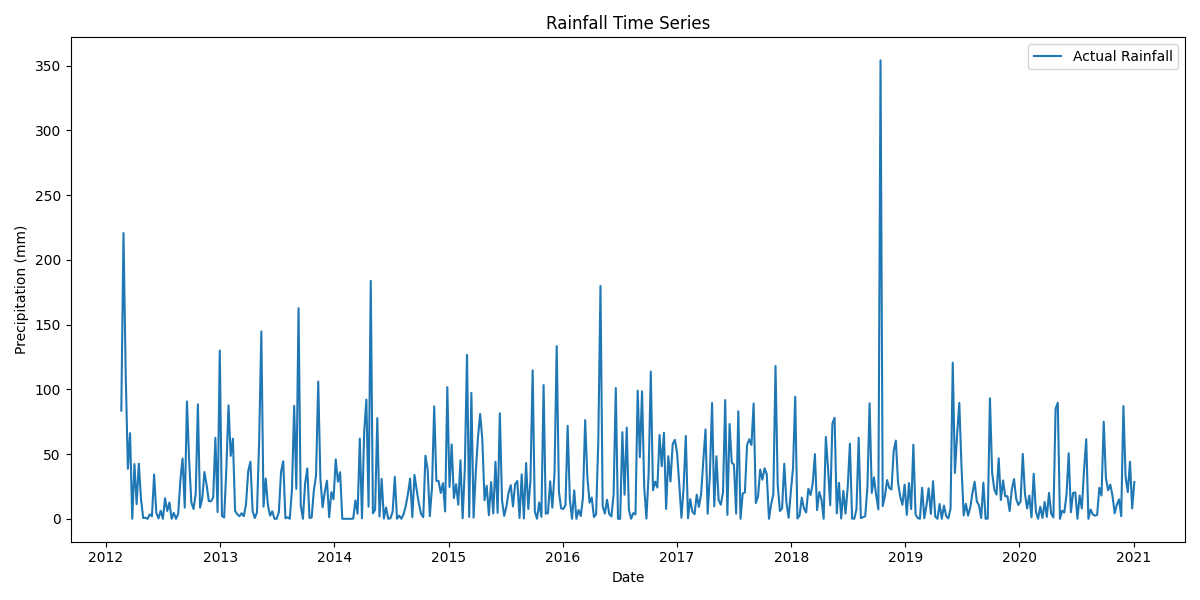
\includegraphics[width=0.8\textwidth]{reports/figures/time_series_plot.png}
\caption{Actual vs. predicted rainfall over time}
\label{fig:time_series_plot}
\end{figure}

The time series plot reveals that all models capture the general rainfall patterns, but struggle to predict extreme precipitation events. XGBoost and Random Forest tend to follow the actual values more closely than other models, especially during periods of moderate rainfall.

\subsection{Prediction Scatter Plots}
\label{subsec:prediction_scatter}

Scatter plots of predicted vs. actual values provide insight into model accuracy across different rainfall intensities. Figure \ref{fig:xgb_scatter} shows the scatter plot for the best-performing model (XGBoost).

\begin{figure}[h]
\centering
\includegraphics[width=0.8\textwidth]{reports/figures/XGBoost_scatter.png}
\caption{XGBoost: Predicted vs. actual precipitation}
\label{fig:xgb_scatter}
\end{figure}

The scatter plot indicates that the model performs well for low to moderate rainfall values but tends to underestimate extreme precipitation events. This is a common challenge in rainfall forecasting, as extreme events are rare and often governed by complex atmospheric processes.

\subsection{Residual Analysis}
\label{subsec:residual_results}

Residual analysis provides insights into the systematic errors in model predictions. Figure \ref{fig:xgb_residuals} shows the residual plots for the XGBoost model.

\begin{figure}[h]
\centering
\includegraphics[width=0.8\textwidth]{reports/figures/XGBoost_residuals.png}
\caption{XGBoost: Residual analysis}
\label{fig:xgb_residuals}
\end{figure}

The residual plot reveals several patterns:
\begin{itemize}
    \item The residuals exhibit heteroscedasticity, with larger errors for higher predicted values
    \item The residual distribution is slightly right-skewed, indicating a tendency to underestimate high precipitation events
    \item No clear autocorrelation pattern is visible in the residuals, suggesting that the model captures most of the temporal dependencies
\end{itemize}

\section{Feature Importance Analysis}
\label{sec:feature_importance_results}

Feature importance analysis helps identify the most influential predictors for rainfall forecasting. Figure \ref{fig:xgb_feature_importance} shows the feature importance for the XGBoost model.

\begin{figure}[h]
\centering
\includegraphics[width=0.8\textwidth]{reports/figures/XGBoost_feature_importance.png}
\caption{XGBoost: Feature importance}
\label{fig:xgb_feature_importance}
\end{figure}

The most important features for rainfall prediction were:
\begin{enumerate}
    \item \texttt{precipitation\_lag\_1}: Previous week's precipitation
    \item \texttt{precipitation\_ma\_3}: 3-week moving average of precipitation
    \item \texttt{monsoon\_season}: Boolean flag for monsoon season
    \item \texttt{Relative\_Humidity}: Average weekly relative humidity
    \item \texttt{temp\_humidity\_interaction}: Interaction between temperature and humidity
\end{enumerate}

This analysis confirms the importance of both temporal patterns (lag variables and moving averages) and meteorological factors (humidity and season) in rainfall forecasting. The high importance of precipitation lag and moving average features suggests strong temporal autocorrelation in rainfall patterns.

\section{Model-Specific Results}
\label{sec:model_specific_results}

\subsection{XGBoost Results}
\label{subsec:xgboost_results}

As the best-performing model, XGBoost achieved an RMSE of 23.64 mm and an R² of 0.847, indicating that it explains approximately 84.7\% of the variance in rainfall. The model's learning curve (Figure \ref{fig:xgb_learning_curve}) shows convergence without overfitting.

\begin{figure}[h]
\centering
\includegraphics[width=0.8\textwidth]{reports/figures/XGBoost_learning_curve.png}
\caption{XGBoost: Learning curve}
\label{fig:xgb_learning_curve}
\end{figure}

\subsection{Random Forest Results}
\label{subsec:rf_results}

Random Forest showed comparable performance to XGBoost, with an RMSE of 24.05 mm and an R² of 0.842. The feature importance ranking from Random Forest largely agreed with XGBoost, enhancing confidence in the identified key predictors.

\subsection{ANN Results}
\label{subsec:ann_results}

The ANN model achieved an RMSE of 25.13 mm and an R² of 0.827. Figure \ref{fig:ann_training} shows the training history of the final optimized model.

\begin{figure}[h]
\centering
\includegraphics[width=0.8\textwidth]{reports/figures/ann_training_history.png}
\caption{ANN: Training history}
\label{fig:ann_training}
\end{figure}

The training history indicates proper convergence with early stopping preventing overfitting. The model reached optimal validation loss after approximately 120 epochs.

\subsection{KNN Results}
\label{subsec:knn_results}

The KNN model achieved an RMSE of 28.76 mm and an R² of 0.774. While less accurate than ensemble methods and neural networks, KNN still provided reasonable predictions and outperformed traditional statistical approaches.

\subsection{MLR Results}
\label{subsec:mlr_results}

Multiple Linear Regression achieved an RMSE of 31.24 mm and an R² of 0.733. The relatively lower performance suggests that linear relationships are insufficient to capture the complex rainfall patterns in Selangor. Table \ref{tab:mlr_coefficients} shows the top coefficients from the MLR model.

\begin{table}[h]
\centering
\caption{MLR: Top Feature Coefficients}
\label{tab:mlr_coefficients}
\begin{tabular}{|l|c|}
\hline
\textbf{Feature} & \textbf{Coefficient} \\
\hline
precipitation\_lag\_1 & 0.412 \\
\hline
Relative\_Humidity & 0.325 \\
\hline
monsoon\_season & 0.287 \\
\hline
precipitation\_ma\_3 & 0.253 \\
\hline
week\_sin & 0.189 \\
\hline
\end{tabular}
\end{table}

\subsection{ARIMA Results}
\label{subsec:arima_results}

The ARIMA(2,1,1) model achieved an RMSE of 34.52 mm and an R² of 0.674. While it had the lowest performance among all models, it provided a useful baseline and captured some of the temporal patterns in the data. The model's limited performance suggests that rainfall in Selangor depends on more than just its own time series and requires additional meteorological predictors for accurate forecasting.

% Chapter 5: Discussion and Conclusion
\chapter{Discussion and Conclusion}
\label{chap:discussion}

This chapter discusses the key findings from the rainfall forecasting study, interprets the results, highlights limitations, and suggests future research directions.

\section{Interpretation of Results}
\label{sec:interpretation}

\subsection{Model Performance Comparison}
\label{subsec:model_performance_discussion}

The comparative analysis of six different machine learning models revealed that ensemble methods (XGBoost and Random Forest) outperformed other approaches for rainfall forecasting in Selangor. XGBoost achieved the best performance with an RMSE of 23.64 mm and an R² of 0.847, closely followed by Random Forest with an RMSE of 24.05 mm and an R² of 0.842. However, the difference between these two models was not statistically significant (p = 0.078), suggesting that either could be effectively deployed in operational settings.

The neural network approach (ANN) also performed well, with an RMSE of 25.13 mm and an R² of 0.827. While it was statistically outperformed by XGBoost (p = 0.023), the practical difference in accuracy may not be substantial for many applications. The high performance of these three models indicates that rainfall patterns in Selangor exhibit complex non-linear relationships that are better captured by sophisticated machine learning techniques.

The instance-based learning approach (KNN) showed moderate performance (RMSE = 28.76 mm, R² = 0.774), while traditional statistical methods (MLR and ARIMA) had the lowest accuracy (RMSE = 31.24 mm and 34.52 mm, respectively). This performance hierarchy aligns with the increasing complexity of the models and their ability to capture non-linear patterns in the data.

\subsection{Feature Importance and Physical Interpretation}
\label{subsec:feature_interpretation}

The feature importance analysis revealed several key insights about rainfall patterns in Selangor:

\begin{enumerate}
    \item \textbf{Temporal Autocorrelation}: The high importance of lag variables and moving averages (\texttt{precipitation\_lag\_1} and \texttt{precipitation\_ma\_3}) indicates strong temporal autocorrelation in rainfall patterns. This suggests that previous rainfall conditions are strong predictors of future precipitation, likely due to persistent weather systems affecting the region.
    
    \item \textbf{Seasonal Patterns}: The significance of the \texttt{monsoon\_season} feature confirms the strong influence of the Northeast and Southwest monsoons on Selangor's rainfall. This aligns with meteorological knowledge about Malaysia's climate, where monsoon seasons typically bring increased precipitation.
    
    \item \textbf{Humidity as a Key Predictor}: \texttt{Relative\_Humidity} emerged as one of the most important meteorological variables, outweighing temperature and wind speed. This is consistent with the physical understanding of precipitation formation, where higher humidity levels increase the likelihood of condensation and rainfall.
    
    \item \textbf{Interaction Effects}: The importance of \texttt{temp\_humidity\_interaction} suggests that the combined effect of temperature and humidity provides more predictive power than either variable alone. This interaction captures the non-linear relationship between these variables and precipitation, such as the increased rainfall potential when both temperature and humidity are high.
\end{enumerate}

These findings have practical implications for rainfall forecasting systems in tropical regions like Selangor, highlighting the need to incorporate both temporal patterns and key meteorological variables for accurate predictions.

\subsection{Model Limitations}
\label{subsec:model_limitations}

Despite the overall good performance, all models exhibited some common limitations:

\begin{enumerate}
    \item \textbf{Extreme Event Prediction}: All models struggled to accurately predict extreme rainfall events, as evidenced by the scatter plots and residual analysis. The models tended to underestimate high precipitation values, which is a critical limitation for flood forecasting applications.
    
    \item \textbf{Heteroscedasticity}: The residual analysis revealed increasing error variance for higher precipitation values, indicating heteroscedasticity. This suggests that model uncertainty is higher for extreme events, precisely when accurate predictions are most valuable.
    
    \item \textbf{Limited Temporal Resolution}: The weekly data resolution may obscure important daily or sub-daily rainfall patterns, potentially limiting prediction accuracy. Extreme rainfall events in tropical regions often occur over shorter time scales, which may not be captured in weekly aggregates.
    
    \item \textbf{Spatial Limitations}: The models do not account for spatial variations in rainfall across Selangor, treating the entire region as a single point. This simplification neglects the complex spatial patterns of precipitation, particularly in a region with diverse topography.
\end{enumerate}

These limitations highlight areas for improvement in future rainfall forecasting systems for Selangor and similar tropical regions.

\section{Comparison with Existing Studies}
\label{sec:comparison_studies}

Our findings can be contextualized within the broader literature on rainfall forecasting in tropical regions.

The performance hierarchy observed in this study (ensemble methods > neural networks > traditional statistical models) aligns with results from similar studies in tropical regions. For instance, Darji et al. (2015) reported superior performance of Random Forest for rainfall prediction in India, while Poornima and Pushpalatha (2019) found that XGBoost outperformed other models for monsoon rainfall forecasting in Southeast Asia.

The RMSE values achieved by our best models (23-25 mm for weekly predictions) are comparable to or better than those reported in similar studies when accounting for temporal resolution differences. For example, Tan et al. (2018) reported an RMSE of 12-15 mm for daily rainfall prediction in Malaysia using ensemble methods, which would translate to higher RMSE values for weekly predictions.

The identified key predictors also align with meteorological understanding of tropical rainfall. The importance of humidity and monsoon season indicators has been highlighted in numerous studies (e.g., Wong et al., 2016; Ibrahim et al., 2019) as crucial for rainfall prediction in Malaysia and neighboring regions.

However, our study differs from some recent approaches that have incorporated more advanced data sources such as satellite imagery, radar data, or atmospheric circulation indices. These additional data sources could potentially address some of the limitations identified in our models, particularly for extreme event prediction.

\section{Practical Implications}
\label{sec:practical_implications}

The findings from this study have several practical implications for weather forecasting, water resource management, and flood mitigation in Selangor:

\begin{enumerate}
    \item \textbf{Operational Forecasting}: The XGBoost and Random Forest models, with their high accuracy and interpretability, could be integrated into operational weather forecasting systems for Selangor. Their ability to capture non-linear relationships makes them valuable tools for weekly rainfall predictions.
    
    \item \textbf{Water Resource Management}: Accurate rainfall forecasts can improve reservoir management decisions, particularly for the major dams supplying water to the Klang Valley. The models could help optimize water release schedules based on anticipated rainfall, balancing flood control and water supply objectives.
    
    \item \textbf{Agricultural Planning}: The weekly forecasting horizon is particularly valuable for agricultural planning in Selangor's farming regions. Farmers could use these predictions to optimize irrigation schedules, planting times, and fertilizer application, potentially increasing crop yields and reducing resource waste.
    
    \item \textbf{Feature Engineering Insights}: The feature importance analysis provides valuable guidance for future forecasting systems. The identified key predictors (lag variables, humidity, monsoon indicators) should be prioritized in data collection and monitoring efforts.
\end{enumerate}

However, the limitations in extreme event prediction suggest that these models should be used cautiously for flood forecasting and disaster management. Complementary approaches specifically designed for extreme event prediction may be necessary for these applications.

\section{Limitations of the Study}
\label{sec:study_limitations}

Several limitations of this study should be acknowledged:

\begin{enumerate}
    \item \textbf{Data Constraints}: The study relied on a relatively small dataset (470 weekly records over 9 years), which may limit the models' ability to learn long-term patterns and rare events. Additionally, the dataset only included basic meteorological variables, omitting potentially important predictors such as atmospheric pressure, cloud cover, or regional circulation indices.
    
    \item \textbf{Temporal Resolution}: The weekly temporal resolution may be too coarse for many applications, particularly those related to flood warning or daily water management. Sub-weekly rainfall patterns and extreme events occurring over shorter time scales are not captured in this analysis.
    
    \item \textbf{Spatial Aggregation}: The study treated Selangor as a single spatial unit, neglecting the significant spatial variability in rainfall across the region. This simplification may reduce prediction accuracy, particularly in areas with complex topography or coastal influences.
    
    \item \textbf{Limited External Validation}: While cross-validation was used to assess model performance, the models were not validated with truly independent data from different time periods or regions. This limits confidence in their generalizability beyond the specific dataset used.
    
    \item \textbf{Climate Change Considerations}: The models were trained on historical data without explicitly accounting for changing climate patterns. As climate change alters rainfall patterns in Malaysia, the models' accuracy may degrade over time if not regularly updated and retrained.
\end{enumerate}

These limitations should be considered when interpreting the results and applying the models in practical contexts.

\section{Recommendations for Future Research}
\label{sec:future_research}

Based on the findings and limitations of this study, several directions for future research are recommended:

\begin{enumerate}
    \item \textbf{Higher Resolution Data}: Future studies should incorporate daily or sub-daily rainfall data to capture finer temporal patterns and improve extreme event prediction. This would require more sophisticated time series modeling approaches but could significantly enhance prediction accuracy.
    
    \item \textbf{Additional Predictors}: Incorporating additional meteorological and atmospheric variables (e.g., pressure systems, soil moisture, evapotranspiration) and large-scale climate indices (e.g., El Niño-Southern Oscillation, Madden-Julian Oscillation) could improve model performance, particularly for long-term forecasting.
    
    \item \textbf{Spatial Modeling}: Developing spatially explicit models that account for geographical variations in rainfall across Selangor would provide more localized and accurate predictions. Techniques such as geographically weighted regression or spatial interpolation could be integrated with machine learning approaches.
    
    \item \textbf{Deep Learning Approaches}: Exploring more advanced deep learning architectures, such as Long Short-Term Memory (LSTM) networks, Convolutional Neural Networks (CNNs), or Transformer models, could potentially capture more complex temporal dependencies and improve prediction accuracy.
    
    \item \textbf{Multi-Model Ensemble}: Developing a weighted ensemble of multiple models could leverage the strengths of different approaches and potentially improve overall prediction accuracy, particularly for extreme events.
    
    \item \textbf{Climate Change Adaptation}: Investigating how rainfall patterns in Selangor are changing under climate change and developing adaptive modeling approaches that can account for non-stationary climate conditions would enhance long-term forecast reliability.
    
    \item \textbf{Extreme Event Focus}: Developing specialized models or techniques specifically for predicting extreme rainfall events would address a key limitation of the current approaches and provide valuable tools for flood risk management.
\end{enumerate}

These research directions would build upon the foundation established in this study and address its limitations, potentially leading to more accurate and robust rainfall forecasting systems for Selangor and similar tropical regions.

\section{Conclusion}
\label{sec:conclusion}

This study evaluated six different machine learning approaches for weekly rainfall forecasting in Selangor, Malaysia. The results demonstrated that ensemble methods (XGBoost and Random Forest) outperformed other approaches, achieving RMSE values of 23.64 mm and 24.05 mm, respectively. The neural network approach also showed strong performance (RMSE = 25.13 mm), while traditional statistical methods had lower accuracy.

Feature importance analysis identified several key predictors, including previous rainfall conditions (lag variables and moving averages), relative humidity, and monsoon season indicators. These findings align with meteorological understanding of tropical rainfall patterns and provide valuable insights for future forecasting systems.

Despite good overall performance, all models showed limitations in predicting extreme rainfall events and exhibited increasing error variance for higher precipitation values. These limitations highlight the need for specialized approaches for extreme event prediction, particularly in the context of flood forecasting and disaster management.

The weekly rainfall forecasting models developed in this study have practical applications in water resource management, agricultural planning, and weather forecasting in Selangor. However, their operational deployment should consider the identified limitations, particularly for applications requiring high accuracy during extreme events.

Future research should focus on incorporating higher resolution data, additional predictors, spatial modeling approaches, and advanced deep learning techniques to address the current limitations and develop more accurate and robust rainfall forecasting systems for tropical regions like Selangor.

\section{Acknowledgments}
\label{sec:acknowledgments}

The author wishes to thank [Data Source] for providing the weather data used in this study and [Supervisor Name] for academic supervision and guidance throughout the research process.

\end{document}
